\section{Our Approach}

\begin{figure*}[h]
	\centering
	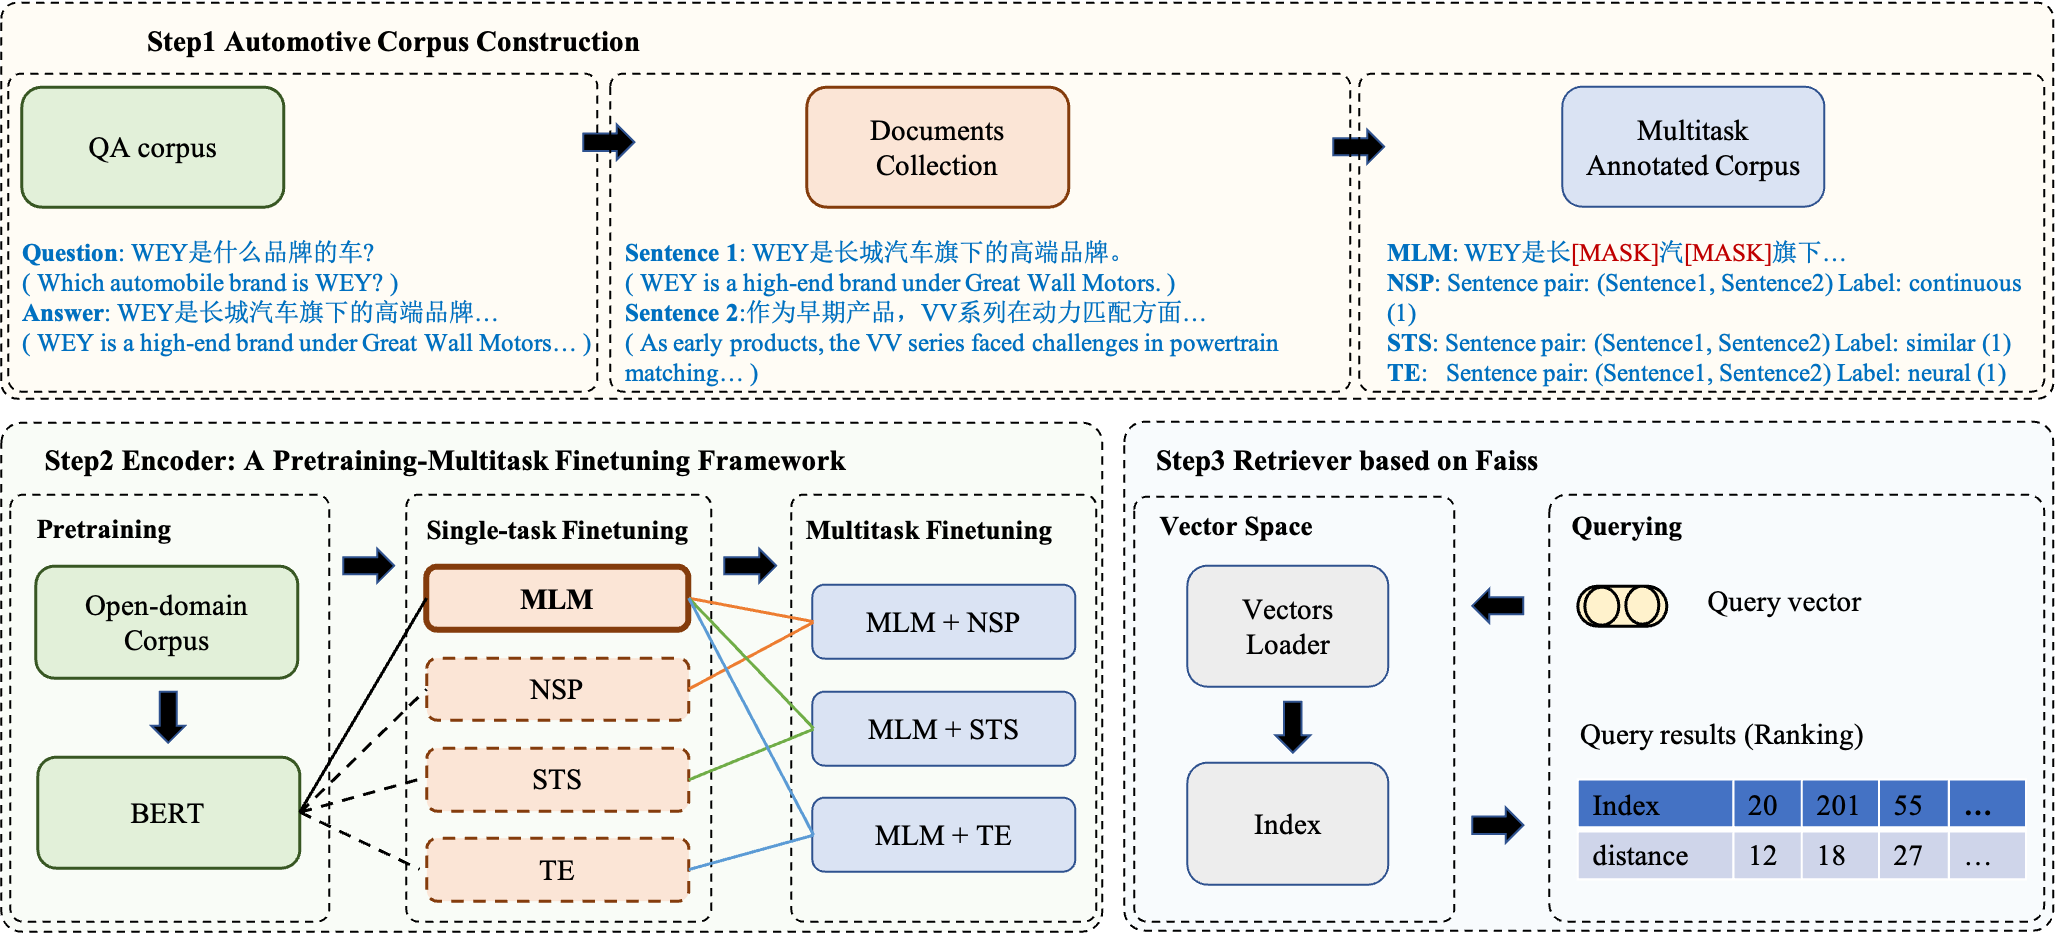
\includegraphics[width=18cm]{overview.png}
	\caption{An overview of our automatic information augmentation framework. \textbf{(a) Step 1}: Interact with ChatGPT to Get Auxiliary Information. \textbf{(b) Step 2}: Distilling the Information and Injecting Them into Context \textbf{(c) Step 3}: Input the Augmented Context into Tagging Model}
	\label{fig:overview}
\end{figure*}   


%\unskip
Existing extractive multi-span question answering models exhibit subpar performance in handling ambiguous words, complex proper nouns (such as film and song titles), numerical values, and long descriptive answers. The main reasons for these shortcomings can be categorized into three aspects:

\textbf{Ambiguous Words}: The real world is replete with words that have a single form but multiple meanings, which heavily depend on the context. For instance, the word ``Cameron" could refer to a famous director or a former British Prime Minister, depending on the context. The specific meanings of such words often appear infrequently in training corpora, making them difficult to learn.

\textbf{Numerical Values}: In contrast to ambiguous words, numerical values have a single meaning but can be represented in various forms. For example, "22.5 billion years" can also be expressed as "cosmic years".

\textbf{Multi-span Answers}: In extractive multi-span question answering tasks, the model needs to grasp the overall relationship of multi-span answers in the context, such as parallelism and progression.These challenges require the model to possess a high level of comprehensive understanding ability and knowledge about language and the world. 

Leveraging large language models to parse question-answering data and inject auxiliary knowledge into the model can promote the integration of the model's latent world knowledge and specific domain knowledge in the paragraph, thereby enhancing the model's performance. Thus, we use GPT-3.5-turbo to generate entity annotations, entity association analysis, and content continuation for each question-answering paragraph as auxiliary information for the model:

\textbf{Context Supplementary}: By inserting explanations of entities in the form of annotations after the main entities or concept words in the question and paragraph, this method helps the model capture the actual meaning of ambiguous words in specific contexts. It provides direct information prompts for low-frequency meanings or low-frequency words, achieving entity or concept alignment in the question-answering system.

\textbf{Context Enrichment}: By integrating entity association analysis and content continuation with the original question-answering text to form new paragraphs based on knowledge enhancement, this method captures the inherent associations between words or entity concepts with the same meaning but different forms. On one hand, it parses the logical relationships between other entities using entity relationship analysis. On the other hand, it extends the original paragraph information using content continuation, introducing more external knowledge while helping the model understand the overall content direction of the paragraph, thereby enhancing the model's comprehension ability.


Overall,we design an automated knowledge enhancement method for multi-span question answering tasks, which interacts with large language models based on templates. This method is applicable to all question answering models or frameworks. It is universally applicable to any other downstream tasks that contain paragraph data, without the need for any complex calculations. In the following sections, we will provide a detailed introduction to each specific module of this process.

\subsection{Construction of Prompt Template}
\label{sec:prompt_construction}
\begin{figure*}[h]
	\centering
	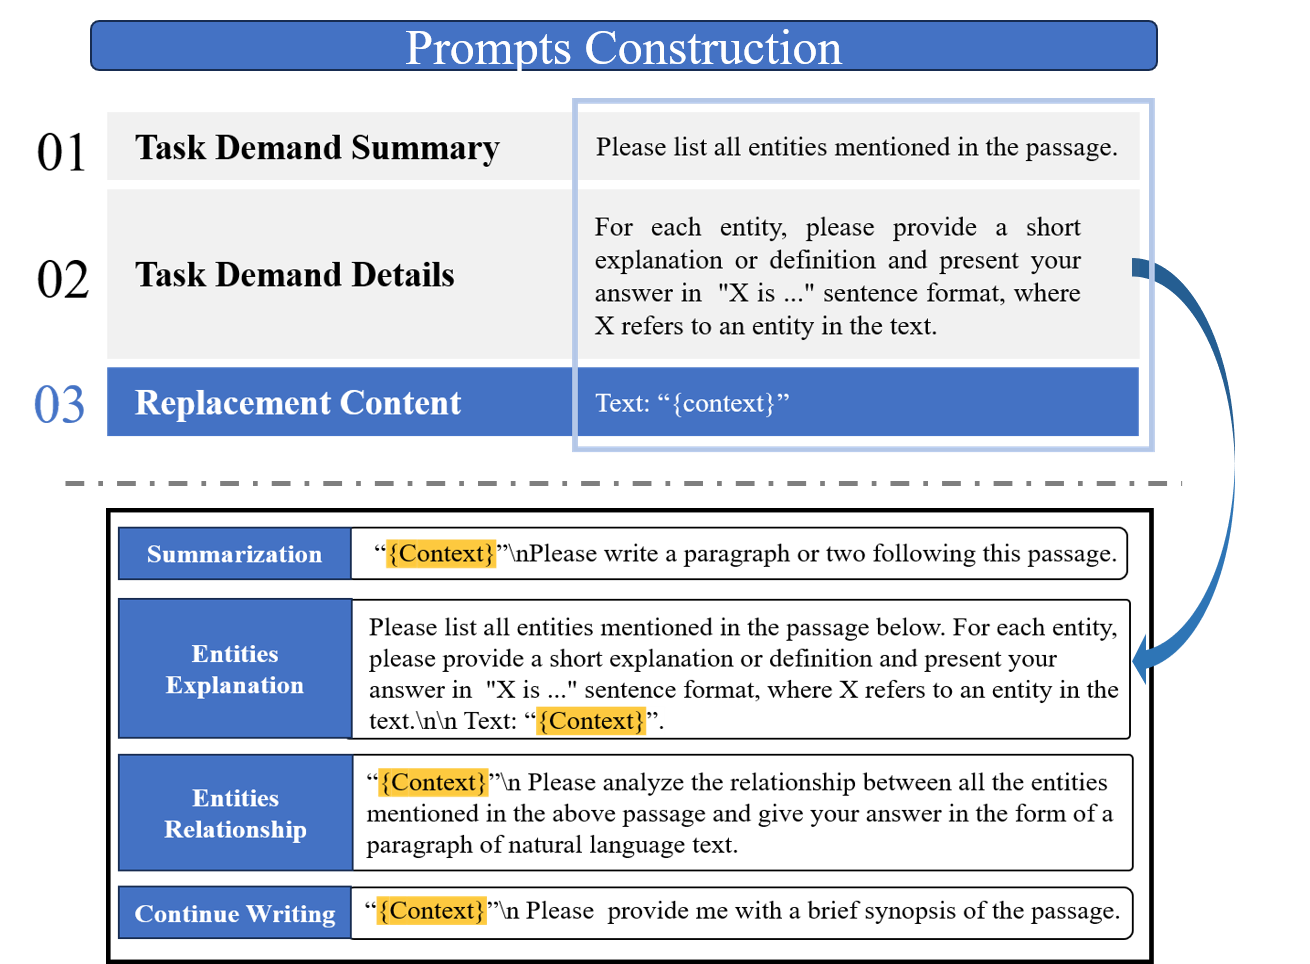
\includegraphics[width=14.5cm]{Prompts_construction.png}
	\caption{Prompt Templates and it's Construction}
	\label{fig:prompt_template}
\end{figure*}   

The quality and format of the content produced by LLMs depends greatly on the prompts. Hence, it is necessary to clarify the format and content requirements of the outputs in advance, and to refine the templates that meet the expectations through extensive evaluation.
For entity relationship parsing and textual continuation, it would be better to ensured that the the output is a natural paragraph, to facilitate the automatic splicing of the enriched knowledge with the initial paragraphs,which is consistent with encoder's natural input format.
Regarding knowledge of entity explanation, the inserted knowledge fusion method requires a parsable and structured outputs for automatic recognition and segmentation of entities and their explanations in post-processing, as well as inserting explanation behind the description of matched entity in initial context.

Concretely, by clearly specifying the form and requirements in the prompts, especially for entity relationship parsing and contextual continuation, which need to be formulated in the form of natural statements, the targeted enhanced knowledge can be obtained more easily.
Furthermore, to obtain well-structured results for complex model interactions, like entity explanations, we utilize a set of corresponding hint templates to construct the process, which has proven to be useful for interactions that require semi-structured answers through verification. 

Eventually, the template is piloted to clarify any ambiguous requirements in the template to confirm an accurate understanding of the LLMs (e.g., adding at the end of the prompt, ``Please return the answer in the following form, being careful not to repeat it: \textbackslash n\textbackslash nA is .....")  In addition, to avoid omission or confusion of requirements due to the length of the prompt text, specific principles should be reiterate in a separate paragraph.

\subsection{Information Injection}

To incorporate enhanced knowledge into the original data (comprising questions and paragraphs) pertaining to entity interpretation, a methodology involving the insertion of explanations is employed. Specifically, the process begins with the automated script parsing of entity interpretation data. This script, on one hand, utilizes regular expressions to analyze the structure of the majority of sentences, while on the other hand, for a limited subset of sentences that deviate from the template specifications, employs Spacy's Semantic Dependency Analysis model to identify entities and their corresponding interpretations.

Upon obtaining the ``Entity-Entity Interpretation" knowledge base for each question-and-answer data, a subsequent scan of the original context is conducted. For each entity that exists in the dataset's library of entities and their explanations, the corresponding explanation is inserted immediately following the entity, enclosed within parentheses. This meticulous approach ensures that the augmented text, enriched with knowledge, retains its natural sentence or paragraph flow. For instance, a resulting sentence might appear as follows: ``How long does it take for the Milky Way (Milky Way: The galaxy that contains our Solar System and is home to billions of stars.) to rotate?" 

\label{sec:information_injection}
\begin{figure*}[h]
	\centering
	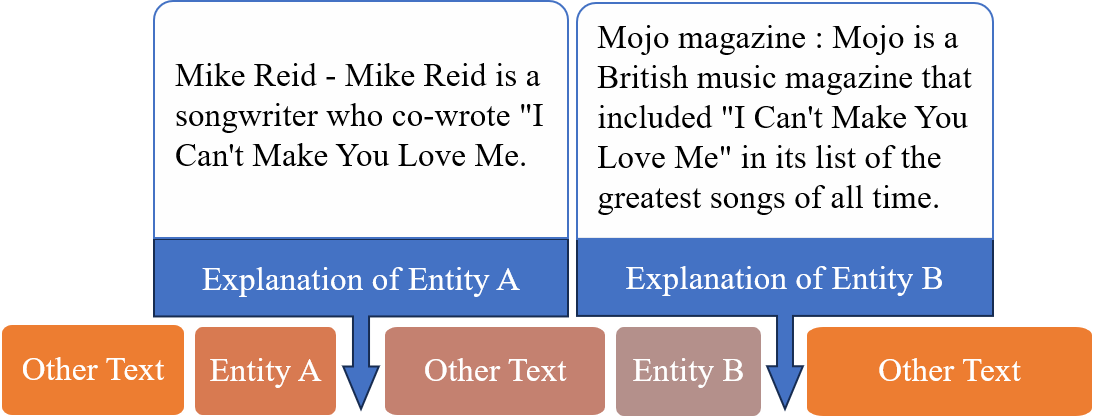
\includegraphics[width=10cm]{EntityInsert.png}
	\caption{The Process of Inserting Entity Explanation into Context}
	\label{fig:entity_insertion}
\end{figure*}

For the incorporation of enhanced knowledge related to entity relationship analysis and content continuation, a method of random slicing and concatenation based on length ratios is employed to infuse the augmented knowledge into the original paragraphs. Initially, the ratio of the average length of the augmented knowledge text to that of the original paragraph is calculated. Subsequently, at the model's input layer, the original input data is segmented into text fragments of length of \textit{512 * average original length / (average original length + average augmented text length)}, and the augmented text is also segmented into text fragments of length of  \textit{512 * average augmented text length / (average original length + average augmented text length)}. Then, random selections of augmented text fragments are made and concatenated into the middle of each original text fragment. Finally, this concatenated longer text is fed into the model in a sliding manner to ensure comprehensive interaction between the original data and the augmented data at lower layers of the model, as illustrated in Figure~\ref{fig:random_concatenate}.



\begin{figure*}[h]
	\centering
	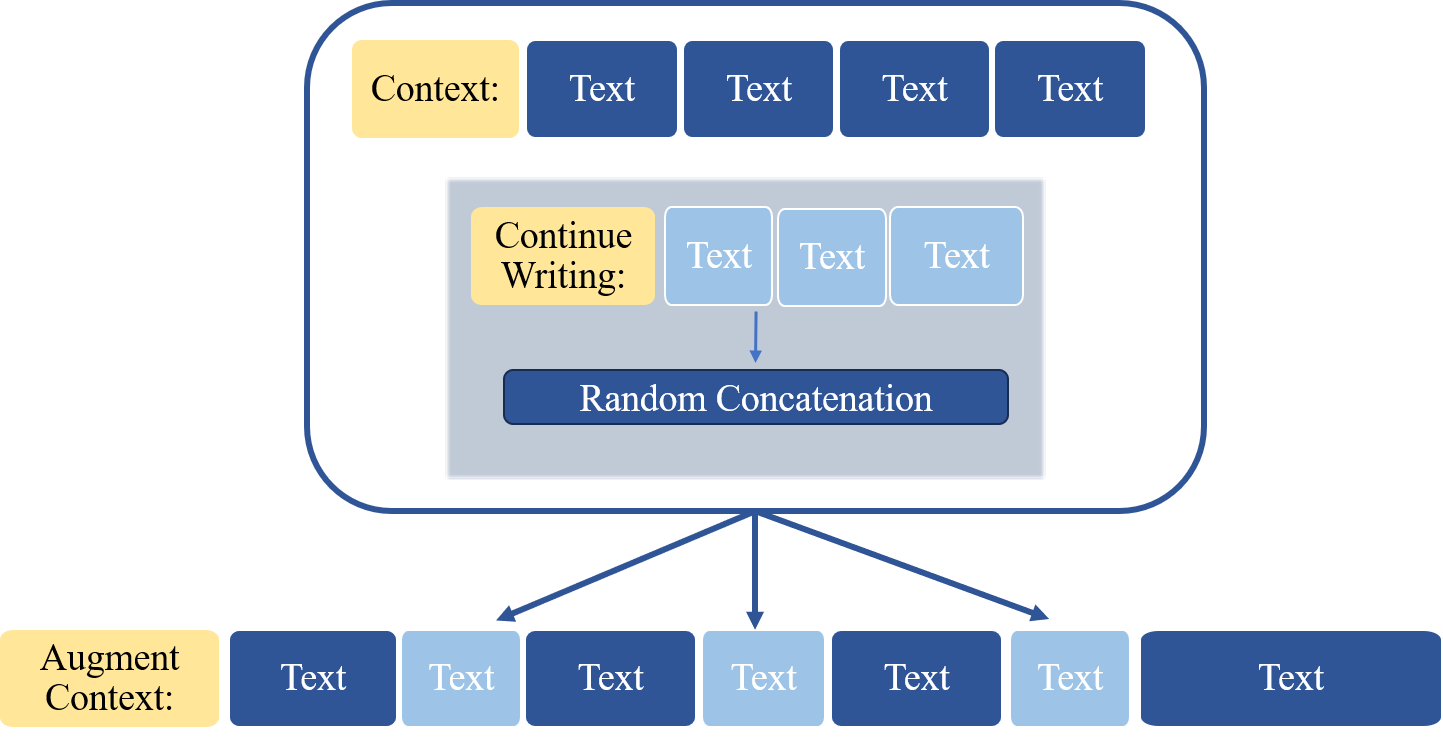
\includegraphics[width=10cm]{RandomConcat.png}
	\caption{The Process of Concatenation of Original Context and Auxiliary Information}
	\label{fig:random_concatenate}
\end{figure*}  

\subsection{Information Integration}
\label{sec:information_integration}
In addition to the aforementioned three types of information, we seek more valuable enhanced information by requesting summaries for each question-context pair from Large Language Models (LLMs). We then extract entities mentioned in the summaries to capture those highly relevant to the core context. Moreover, recognizing the intrinsic connection between entity explanation and entity relationship parsing, we categorize them as complementary information for context enrichment, with context continuation serving as supplementary information. This approach aims to augment the model's internal text-parsing knowledge with external world knowledge through enhanced information. 

To further investigate the efficacy of multi-information integration, leveraging enhanced information derived from Large Language Models (LLMs), we employ two distinct approaches to combine entity knowledge and context continuity. The first approach involves the incorporation of all information within the original context, with each type of information undergoing individualized knowledge injection. The second approach, referred to as "bagging," treats models trained on diverse information sources as voters. For each query, we employ all model predictions for token-level BIO labeling within the context, determining the final prediction through a majority vote. In cases of tie-breaking, we prioritize the logits' magnitude to ascertain the ultimate prediction.

